%%%%%%%%%%%%%%%%%%%%%%%%%%%%%%%%%%%%

\section{2.2. Probabilidade Condicional}

%%%%%%%%%%%%%%%%%%%%%%%%%%%%%%%%%%%%

\subsection{Probabilidades marginais e conjuntas}

%%%%%%%%%%%%%%%%%%%%%%%%%%%%%%%%%%%%

\begin{frame}
\frametitle{Tipos de tratamento para vício em cocaína}
\justifying
Pesquisadores distribuíram aleatoriamente 72 usuários de cocaína em três grupos de tratamento contra o vício: um grupo recebe o medicamento desipramina (antidepressivo), outro o lítio (tratamento padrão para cocaína) e o último grupo recebe um placebo. Os resultados do estudo estão resumidos abaixo.

{\small
\begin{center}
\begin{tabular}{l | c c | c}
			& 		& Não 		&  \\
			& Recaída	& Recaída	& total \\
\hline
desipramina	& 10		& 14		& 24 \\
lítio		& 18		& 6		& 24 \\
placebo		& 20		& 4		& 24 \\
\hline
total			& 48		& 24		& 72
\end{tabular}
\end{center}
}
\justifying
\ct{\webURL{http://www.oswego.edu/~srp/stats/2_way_tbl_1.htm}}

\end{frame}

%%%%%%%%%%%%%%%%%%%%%%%%%%%%%%%%%%%%

\begin{frame}
\frametitle{Probabilidade Marginal}
\justifying
\dq{Qual é a probabilidade de um paciente ter uma recaída?}

{\small
\begin{center}
\begin{tabular}{l | c c | c}
			& Ter		& Não ter 		&  \\
			& recaída	& recaída	& total \\
\hline
desipramina	& 10		& 14		& 24 \\
lítio		& 18		& 6		& 24 \\
placebo		& 20		& 4		& 24 \\
\hline
total			& \only<1>{48}\only<2->{\red{48}}		& 24		&  \only<1>{72}\only<2->{\red{72}}
\end{tabular}
\end{center}
}
\justifying
\onslide<2->{P(Ter uma recaída) = $\frac{48}{72} \approx 0.67$} \\

\end{frame}

%%%%%%%%%%%%%%%%%%%%%%%%%%%%%%%%%%%%

\begin{frame}
\frametitle{Probabilidade conjunta}
\justifying
\dq{Qual é a probabilidade de um paciente receber o antidepressivo (desipramina)? \underline{e} ter uma recaída?}

{\small
\begin{center}
\begin{tabular}{l | c c | c}
			& 		& não 		&  \\
			& recaída	& recaída	& total \\
\hline
desipramina	& \only<1>{10} \only<2->{\red{10}}		& 14		& 24 \\
lítio		& 18		& 6		& 24 \\
placebo		& 20		& 4		& 24 \\
\hline
total			& 48	& 24		&  \only<1>{72} \only<2->{\red{72}}
\end{tabular}
\end{center}
}
\justifying
\onslide<2->{P(recaída e desipramina) = $\frac{10}{72} \approx 0.14$} \\

\end{frame}

%%%%%%%%%%%%%%%%%%%%%%%%%%%%%%%%%%%%

\subsection{Definindo probabilidade condicional}

%%%%%%%%%%%%%%%%%%%%%%%%%%%%%%%%%%%%

\begin{frame}
\frametitle{Probabilidade Condicional}
\justifying
\formula{Probabilidade Condicional}{
A probabilidade do evento $A$ dado que o evento $B$ ocorreu é calculada como
\[ P(A|B) = \frac{P(A~e~B)}{P(B)} = \frac{P(A~\cap~B)}{P(B)} \]
}

\pause

\twocol{0.5}{0.5}
{
{\small
\begin{center}
\begin{tabular}{l | c c | c}
			& 		& não 		&  \\
			& recaída	& recaída	& total \\
\hline
desipramina	& 10		& 14		& 24 \\
lítio		& 18		& 6		& 24 \\
placebo		& 20		& 4		& 24  \\
\hline
total			& 48		& 24		&  72
\end{tabular}
\end{center}
}
}
{
\begin{eqnarray*}
&&P(\mbox{recaída} |  \mbox{desipramina}) \\
&&= \frac{P(\mbox{recaida} ~e ~\mbox{desipramina})}{P(\mbox{desipramina})} \\
\pause
&&= \frac{10 / 72}{24 / 72} \\
\pause
&&= \frac{10}{24} \\
\pause
&&= 0.42
\end{eqnarray*}
}

\end{frame}

%%%%%%%%%%%%%%%%%%%%%%%%%%%%%%%%%%%%

\begin{frame}
\frametitle{Probabilidade Condicional (cont.)}
\justifying
\dq{Se sabemos que um paciente recebeu o antidepressivo (desipramina), qual é a probabilidade de que ele tenha uma recaída e volte a usar a droga?}

{\small
\begin{center}
\begin{tabular}{l | c c | c}
			& 		& não 		&  \\
			& recaída	& recaída	& total \\
\hline
\rowcolor[gray]{.7}
desipramina	& \only<1>{10} \only<2->{\red{10}}			& 14		& \only<1>{24} \only<2->{\red{24}} \\
lítio		& 18		& 6		& 24 \\
placebo		& 20 		& 4		& 24  \\
\hline
total			& 48	& 24		&  72
\end{tabular}
\end{center}
}
\justifying
\onslide<2->{P(recaída $|$  desipramina) = $\frac{10}{24} \approx 0.42$} \\

\onslide<3->{
$\:$ \\
P(recaída $|$  lítio) = $\frac{18}{24} \approx 0.75$ \\
P(recaída $|$  placebo) = $\frac{20}{24} \approx 0.83$ \\
}

\end{frame}

%%%%%%%%%%%%%%%%%%%%%%%%%%%%%%%%%%%%

\begin{frame}
\frametitle{Probabilidade Condicional (cont.)}
\justifying
\dq{Se sabemos que um paciente teve uma recaída, qual é a probabilidade de terem recebido o tratamento com o antidepressivo (desipramina)?}

{\small
\begin{center}
\begin{tabular}{l | >{\columncolor[gray]{0.7}[0pt]}c c | c}
			& 		& não 		&  \\
			& recaída	& recaída	& total \\
\hline
desipramina	& \only<1>{10} \only<2->{\red{10}}			& 14		& 24 \\
lítio		& 18		& 6		& 24 \\
placebo		& 20		& 4		& 24  \\
\hline
total			& \only<1>{48} \only<2->{\red{48}}	& 24		&  72
\end{tabular}
\end{center}
}
\justifying
\onslide<2->{P(desipramina $|$  recaída) = $\frac{10}{48} \approx 0.21$} \\

\onslide<3->{
$\:$ \\
P(lítio $|$  recaída) = $\frac{18}{48} \approx 0.375$ \\
P(placebo $|$  recaída) = $\frac{20}{48} \approx 0.42$ \\
}

\end{frame}

%%%%%%%%%%%%%%%%%%%%%%%%%%%%%%%%%%%%

\subsection{Regra geral de multiplicação}

%%%%%%%%%%%%%%%%%%%%%%%%%%%%%%%%%%%%

\begin{frame}
\frametitle{Regra geral da multiplicação}

\begin{itemize}
\justifying
\item Anteriormente, vimos que, se dois eventos são independentes, a probabilidade conjunta (eles ocorrerem simultaneamente) é simplesmente o produto de suas probabilidades. Se os eventos não forem considerados independentes, a probabilidade conjunta é calculada de forma ligeiramente diferente.

\pause
\justifying
\item Se $A$ e $B$ representam dois eventos quaisquer, então
\formula{\[ P(A~e~B) = P(A|B) \times P(B) \]}
\formula{\[ P(A\cap B) = P(A|B) \times P(B) \]}

\justifying
Note que a equação acima é simplesmente a fórmula da probabilidade condicional, rearranjada.
\pause
\justifying
\item É útil pensar em $A$ como resultado e o evento $B$ como condição.

\end{itemize}

\end{frame}

%%%%%%%%%%%%%%%%%%%%%%%%%%%%%%%%%%%%

\subsection{Independência e probabilidade condicional}

%%%%%%%%%%%%%%%%%%%%%%%%%%%%%%%%%%%%

\begin{frame}
\frametitle{Probabilidade condicional}
\justifying
Considere a seguinte distribuição (hipotética) de número de alunos aprovados e reprovados nos cursos de estatística e física:

{\small
\begin{center}
\begin{tabular}{l | c c | c}

			& Estatística	& Física	& total \\
\hline
Aprovado		& 30		& 20		& 50 \\
reprovado			& 30		& 20		& 50 \\
\hline
total			& 60		& 40		& 100
\end{tabular}
\end{center}
}

\pause

\begin{itemize}
\justifying
\item A probabilidade de que um estudante selecionado aleatoriamente seja do curso da estatística é \pause $\frac{60}{100} = 0.6$. 
\end{itemize}
\end{frame}
%%%%%%%%%%%%%%%%%%%%%%%%%%%%%%%%%%%%

\begin{frame}
\frametitle{Probabilidades de eventos independentes e probabilidade condicional}
\pause
\justifying
\begin{itemize}
\justifying
\item A probabilidade de que um estudante selecionado aleatoriamente seja do curso de estatística, dado que ele foi aprovado na disciplina. \pause $\frac{30}{50} = 0.6$. 

\pause
\justifying
\item Desde a $P(Estatística| Reprovado)$ também é igual a 0,6; a aprovação ou reprovação do aluno não trazem informação sobre o curso do aluno, logo o aluno ser da estatística ou da física é depende da reprovação ou aprovação na disciplina: P(Estatística $|$ Aprovado) = P(Estatística).

\end{itemize}

\end{frame}

%%%%%%%%%%%%%%%%%%%%%%%%%%%%%%%%%%%%

\begin{frame}
\frametitle{Probabilidades de eventos independentes e probabilidade condicional (cont.)}
\justifying
Genericamente, se $P(A|B) = P(A)$ então os eventos $A$ e $B$ são ditos independentes.

\pause

\begin{itemize}
\justifying
\item Conceitualmente: dar $B$ não nos diz nada sobre $A$.

\pause
\justifying
\item Matematicamente: sabemos que se eventos $A$ e $B$ são independentes, $P(A~e~B) = P(A) \times P(B)$. Então,
\[ P(A|B) = \frac{P(A~e~B)}{P(B)} = \frac{P(A) \times P(B)}{P(B)} = P(A) \]


\justifying
\item Em tabelas de contingência essa propriedade deve ser válida para todas as combinações de resultados.


\end{itemize}

\end{frame}

%%%%%%%%%%%%%%%%%%%%%%%%%%%%%%%%%%%%

\subsection{Diagramas de árvore}

%%%%%%%%%%%%%%%%%%%%%%%%%%%%%%%%%%%%

%%%%%%%%%%%%%%%%%%%%%%%%%%%%%%%%%%%%

\begin{frame}
\frametitle{Pesquisa sobre câncer da mama}

\begin{itemize}
\justifying
\item A Sociedade Americana de Câncer estima que cerca de 1,7\% das mulheres têm câncer de mama. \\
{\small\webURL{http://www.cancer.org/cancer/cancerbasics/cancer-prevalence}}
\justifying
\item Susan G. Komen, da Fundação Cura, afirma que a mamografia identifica corretamente 78\% das mulheres que realmente têm câncer de mama. \\
{\small\webURL{http://ww5.komen.org/BreastCancer/AccuracyofMammograms.html}}
\justifying
\item Um artigo publicado em 2003 sugere que até 10\% de todas as mamografias resultam em falsos positivos para pacientes que não têm câncer. \\{\small \webURL{http://www.ncbi.nlm.nih.gov/pmc/articles/PMC1360940}}

\end{itemize}

\vfill
\justifying
\Note{Essas porcentagens são aproximadas.}

\end{frame}

%%%%%%%%%%%%%%%%%%%%%%%%%%%%%%%%%%%

\begin{frame}
\frametitle{Invertendo probabilidades}
\justifying
\dq{Quando uma paciente passa por um exame de câncer de mama, há duas afirmações concorrentes: a paciente tinha câncer e a paciente não tem câncer. Se uma mamografia produzir um resultado positivo, qual é a probabilidade da paciente realmente ter câncer??}

\pause

\twocol{0.7}{0.3}{
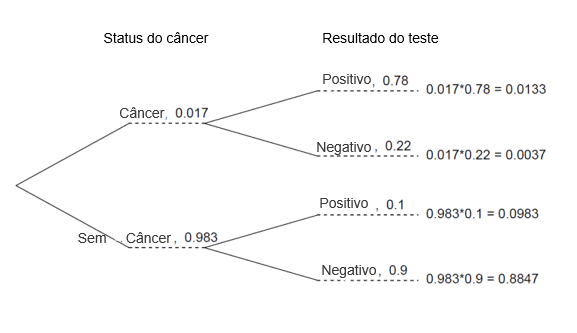
\includegraphics[width=0.9\textwidth]{2-2_conditional_probability/cancer_tree_first.png} 
}
{
\pause
{\footnotesize
\begin{eqnarray*}
&&P(C | +) \\
\pause
&&= \frac{P(C~e~+)}{P(+)} \\
\pause
&&= \frac{0.0133}{0.0133 + 0.0983} \\
\pause
&&= 0.12
\end{eqnarray*}
}
}

\pause
\justifying
\Note{Diagramas de árvores são úteis para inverter probabilidades: nos são dados $P(+|C)$ e pediu por $P(C|+)$.}

\end{frame}

%%%%%%%%%%%%%%%%%%%%%%%%%%%%%%%%%%%

\begin{frame}
\frametitle{Prática}
\justifying
\pq{Suponha que uma mulher que faça o teste uma vez obtenha um resultado positivo, se ela fizer o teste novamente, qual é a probabilidade de que essa mulher tenha câncer se essa segunda mamografia também produzir um resultado positivo?}

\twocol{0.2}{0.7}
{
\begin{enumerate}[(a)]
\item 0.0936
\item 0.088
\item 0.48
\solnMult{0.52}
\end{enumerate}
}
{
\solnGr{\only<2->{
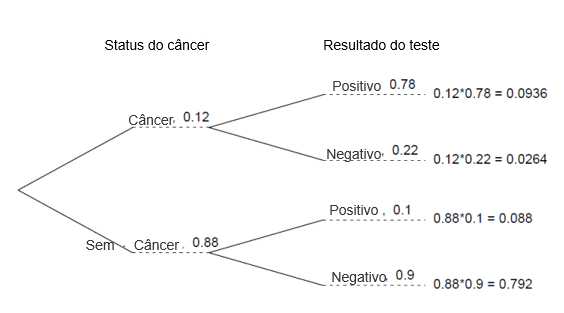
\includegraphics[width=\textwidth]{2-2_conditional_probability/cancer_tree_second.png} 
}}
}

\soln{\only<3->{
{\small \[P(C | +) = \frac{P(C~e~+)}{P(+)} = \frac{0.0936}{0.0936+0.088} = 0.52\]}
}}

\end{frame}

%%%%%%%%%%%%%%%%%%%%%%%%%%%%%%%%%%%

\subsection{Teorema de Bayes}

%%%%%%%%%%%%%%%%%%%%%%%%%%%%%%%%%%%%

\begin{frame}
\frametitle{Teorema de Bayes}

\begin{itemize}
\justifying
\item A fórmula de probabilidade condicional que vimos até agora é um caso especial do Teorema de Bayes, que também é aplicável mesmo quando os eventos têm mais de dois resultados.

\pause 
\begin{center}
    

\item \hl{Teorema de Bayes:}
\formula{
\[ P(resultado~A_1~da~variável~1~|~resultado~B~da~variável~2) \]
\[ = \frac{P(B|A_1)P(A_1)}{P(B|A_1)P(A_1) + P(B|A_2)P(A_2) + \cdots + P(B|A_k)P(A_k)} \]
}
em que $A_2$, $\cdots$, $A_k$ representam todos os outros resultados possíveis da variável 1.
\end{center}
\end{itemize}

\end{frame}

%%%%%%%%%%%%%%%%%%%%%%%%%%%%%%%%%%%

\begin{frame}
\frametitle{Atividade: invertendo probabilidades}
\justifying
\app{{\footnotesize Um modelo epidemiológico comum para a disseminação de doenças é o modelo SIR, onde a população é dividida em três grupos: Suscetível, Infectado e Recuperado. Este é um modelo razoável para doenças como catapora, onde uma única infecção geralmente fornece imunidade a infecções subsequentes. Às vezes, essas doenças também podem ser difíceis de detectar.
\vspace{2mm} \\
\justifying
Imagine uma população no meio de uma epidemia onde 60\% da população é considerada suscetível, 10\% está infectada e 30\% é recuperada. O único teste para a doença tem precisão de 95\% para indivíduos suscetíveis, 99\% para indivíduos infectados, mas 65\% para indivíduos recuperados. (Nota: Neste caso, precisão significa retornar um resultado negativo para indivíduos suscetíveis e recuperados e um resultado positivo para indivíduos infectados). \vspace{2mm} \\
Desenhe uma árvore de probabilidade para refletir as informações fornecidas acima. Se o indivíduo testou positivo, qual é a probabilidade de ele realmente estar infectado?
}}

\end{frame}

%%%%%%%%%%%%%%%%%%%%%%%%%%%%%%%%%%%

\begin{frame}
\frametitle{Atividade: invertendo probabilidades(cont.)}

\vspace{-0.5cm}

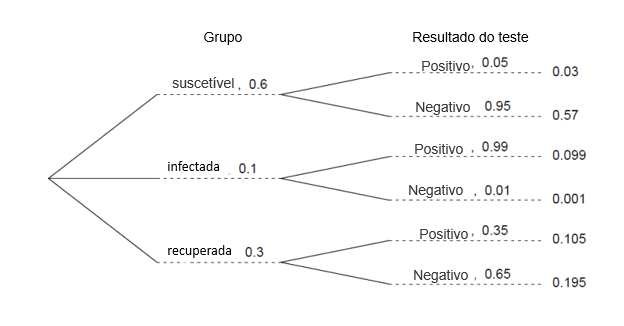
\includegraphics[width=\textwidth]{2-2_conditional_probability/sir_tree.png} 

\pause

\[ P(inf | +) = \frac{P(inf~e~+)}{P(+)} = \frac{0.099}{0.03 + 0.099 + 0.105} \approx 0.423 \]


\end{frame}

%%%%%%%%%%%%%%%%%%%%%%%%%%%%%%%%%%%%

